\section{ベクトルとその演算}

\subsection{ベクトルの定義}

\emph{ベクトル}とは、いくつかの実数を順序付けて並べたものです。これらの数を\emph{成分}と呼びます。$n$個の成分を持つベクトルを\emph{$n$次元ベクトル}といい、縦に並べた\emph{列ベクトル}として表します。また、横に並べた\emph{行ベクトル}として表すこともあります。
\[\bm{v} = \begin{pmatrix} v_1 \\ v_2 \\ \vdots \\ v_n \end{pmatrix} \quad (v_1, v_2,\ldots,v_n\in\mathbb{R})\]
\[\bm{w} = (w_1 \ w_2 \ \dots \ w_n) \quad (w_1, w_2,\ldots,w_n\in\mathbb{R})\]

\begin{ex}
2次元ベクトル $\bm{a} = \begin{pmatrix} 3 \\ 2 \end{pmatrix}$ は、第1成分が3、第2成分が2であることを示します。
また、2次元の行ベクトル $\bm{b} = (1 \ 5)$ は、第1成分が1、第2成分が5であることを示します。
\end{ex}

\begin{dfn}[ベクトルの等しさ] \label{vector_equality}
2つのベクトル$\bm{a}=\begin{pmatrix} a_1 \\ \vdots \\ a_n \end{pmatrix}$と$\bm{b}=\begin{pmatrix} b_1 \\ \vdots \\ b_n \end{pmatrix}$が等しいとは、それらの対応するすべての成分が等しいことをいいます。すなわち、$a_i=b_i$がすべての$i=1,\ldots,n$について成り立つとき、$\bm{a}=\bm{b}$と定義します。
\end{dfn}

\begin{ex}
$\begin{pmatrix} x \\ y \end{pmatrix} = \begin{pmatrix} 5 \\ -3 \end{pmatrix}$ならば、$x=5$ かつ $y=−3$ です。
\end{ex}

\begin{dfn}[零ベクトル] \label{vector_zero}
すべての成分が $0$ のベクトルを\emph{零ベクトル}といい、$\bm{0}$ で表します。
\end{dfn}

\begin{ex}
2次元の零ベクトルは$\bm{0} = \begin{pmatrix} 0 \\ 0 \end{pmatrix}$
\end{ex}

\emph{ベクトルの幾何学的解釈}: ベクトルは、その代数的な定義(成分の羅列)とは別に、\emph{空間内の点の位置や原点からその点へ向かう有向線分(矢印)}として直感的に理解することができます。\emph{この矢印の長さがベクトルの大きさを、矢印の方向がベクトルの向き}を表します。

\begin{ex}
ベクトル$\bm{a} = \begin{pmatrix} 3 \\ 2 \end{pmatrix}$は、原点$(0,0)$から点$(3,2)$へ向かう矢印として図示できます。この図示によって、ベクトルの持つ「移動」や「方向」といった意味合いを視覚的に捉えることができます。
\begin{center}
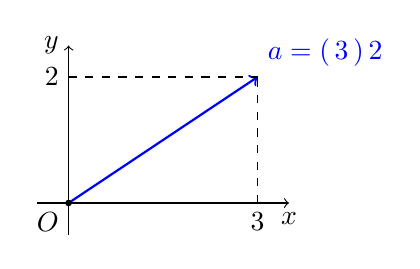
\begin{tikzpicture}[scale=0.8]
    \draw[->] (-0.5,0) -- (3.5,0) node[below] {$x$};
    \draw[->] (0,-0.5) -- (0,2.5) node[left] {$y$};
    \draw[thick, ->, blue] (0,0) -- (3,2) node[above right] {$\bm{a}=\begin{pmatrix} 3 \\ 2 \end{pmatrix}$};
    \draw[dashed] (3,0) node[below] {$3$} -- (3,2);
    \draw[dashed] (0,2) node[left] {$2$} -- (3,2);
    \fill (0,0) circle (1.5pt) node[below left] {$O$};
\end{tikzpicture}
\end{center}
\end{ex}

\subsection{ベクトルの演算の定義と性質}

\subsubsection{ベクトルの和(足し算)}

\begin{dfn}[ベクトルの和] \label{vector_sum}
同じ次元のベクトル$\bm{a}=\begin{pmatrix} a_1 \\ \vdots \\ a_n \end{pmatrix}$と$\bm{b}=\begin{pmatrix} b_1 \\ \vdots \\ b_n \end{pmatrix}$の和$\bm{a}+\bm{b}$は、対応する成分同士を足し合わせることで定義されます。
\[\bm{a} + \bm{b} = \begin{pmatrix} a_1 + b_1 \\ a_2 + b_2 \\ \vdots \\ a_n + b_n \end{pmatrix}\]
\end{dfn}

\begin{ex}
$\begin{pmatrix} 3 \\ 2 \end{pmatrix} + \begin{pmatrix} 1 \\ 4 \end{pmatrix} = \begin{pmatrix} 3 + 1 \\ 2 + 4 \end{pmatrix} = \begin{pmatrix} 4 \\ 6 \end{pmatrix}$
\end{ex}

\emph{幾何学的解釈}: ベクトルの和は、\emph{「移動の連続」}として考えることができます。一方のベクトルの終点に他方のベクトルの始点を置いたとき、最初の始点から最後の終点への矢印が和になります(\emph{三角形の法則})。また、始点をそろえて平行四辺形を作ったときの対角線が和のベクトルになります(\emph{平行四辺形の法則})。
\begin{center}
\begin{tikzpicture}
    % 三角形の法則
    \draw[->] (0,0) -- (2,0.5) node[right] {$\bm{a}$};
    \draw[->] (2,0.5) -- (3.5,2.5) node[right] {$\bm{b}$};
    \draw[thick, ->, blue] (0,0) -- (3.5,2.5) node[above left] {$\bm{a}+\bm{b}$};
    \node at (1.75,1.75) [above left=6pt] {三角形の法則};
    % 平行四辺形の法則
    \begin{scope}[shift={(5.5,0)}]
    \draw[->] (0,0) -- (2,0.5) node[right] {$\bm{a}$};
    \draw[->] (0,0) -- (1.5,2) node[left] {$\bm{b}$};
    \draw[dashed] (2,0.5) -- (3.5,2.5);
    \draw[dashed] (1.5,2) -- (3.5,2.5);
    \draw[thick, ->, blue] (0,0) -- (3.5,2.5) node[above right] {$\bm{a}+\bm{b}$};
    \node at (1.75,1.75) [above left=6pt] {平行四辺形の法則};
    \end{scope}
\end{tikzpicture}
\end{center}

\begin{thm}[ベクトルの和の性質] \label{vector_sum_property}
ベクトルの和は、以下の性質を持ちます。
\begin{enumerate}
\item \emph{交換法則}: $\bm{a} + \bm{b} = \bm{b} + \bm{a}$
\item \emph{結合法則}: $(\bm{a} + \bm{b}) + \bm{c} = \bm{a} + (\bm{b} + \bm{c})$
\item \emph{零ベクトルの存在}: 任意のベクトル $\bm{a}$ に対して、$\bm{a} + \bm{0} = \bm{a}$ となる零ベクトル $\bm{0}$ が存在する。
\item \emph{逆ベクトルの存在}: 任意のベクトル $\bm{a}$ に対して、$\bm{a} + (-\bm{a}) = \bm{0}$ となるベクトル $-\bm{a}$ が存在する。ここで、$-\bm{a}$ は $\bm{a}$ の各成分に $-1$ を掛けたベクトル $\begin{pmatrix} -a_1 \\ \vdots \\ -a_n \end{pmatrix}$ です。
\end{enumerate}
\begin{proof*}
ここでは、\emph{交換法則}の証明を示します。その他の性質は、同様の方法で成分計算によって証明できます(一部は練習問題とします)。\par
$\bm{a} = \begin{pmatrix} a_1 \\ \vdots \\ a_n \end{pmatrix},\ \bm{b} = \begin{pmatrix} b_1 \\ \vdots \\ b_n \end{pmatrix}$ とする。定義\ref{vector_sum}より、$\bm{a} + \bm{b} = \begin{pmatrix} a_1 + b_1 \\ \vdots \\ a_n + b_n \end{pmatrix}$。実数の足し算は交換法則を満たす($x+y = y+x$)ので、各成分について $a_i + b_i = b_i + a_i$ が成り立つ。よって、$\begin{pmatrix} a_1 + b_1 \\ \vdots \\ a_n + b_n \end{pmatrix} = \begin{pmatrix} b_1 + a_1 \\ \vdots \\ b_n + a_n \end{pmatrix}$。再び定義\ref{vector_sum}より、これは $\bm{b} + \bm{a}$ に等しい。したがって、$\bm{a} + \bm{b} = \bm{b} + \bm{a}$ が成り立つ。(証明終)
\end{proof*}
\end{thm}

\subsection{スカラー倍(定数倍)}

\begin{dfn}[ベクトルのスカラー倍] \label{vector_scalar}
ベクトル $\bm{a} = \begin{pmatrix} a_1 \\ \vdots \\ a_n \end{pmatrix}$ と実数 $k$(\emph{スカラー})の積 $k\bm{a}$ は、ベクトルの各成分に $k$ を掛けることで定義されます。
\[k\bm{a} = \begin{pmatrix} k a_1 \\ k a_2 \\ \vdots \\ k a_n \end{pmatrix}\]
\end{dfn}

\begin{ex}
$2 \begin{pmatrix} 3 \\ 2 \end{pmatrix} = \begin{pmatrix} 2 \times 3 \\ 2 \times 2 \end{pmatrix} = \begin{pmatrix} 6 \\ 4 \end{pmatrix}$
\end{ex}

\emph{幾何学的解釈}: スカラー倍は、ベクトルの\emph{長さを伸縮させたり、向きを反転させたり}する操作です。
\begin{itemize}
\item $k > 0$ なら、元のベクトルと同じ向きで長さが $k$ 倍になります。
\item $k < 0$ なら、元のベクトルと逆向きで長さが $|k|$ 倍になります。
\item $k = 0$ なら、すべての成分が $0$ になるため、\emph{零ベクトル}$\bm{0}$ になります。
\end{itemize}

\begin{thm}[スカラー倍の性質] \label{vector_scalar_property}
スカラー倍は、以下の性質を持ちます。
\begin{enumerate}
\item \emph{結合法則}: $k(l\bm{a}) = (kl)\bm{a}$
\item \emph{分配法則(スカラーについて)}: $(k+l)\bm{a} = k\bm{a} + l\bm{a}$
\item \emph{分配法則(ベクトルについて)}: $k(\bm{a}+\bm{b}) = k\bm{a} + k\bm{b}$
\item \emph{単位元}: $1\bm{a} = \bm{a}$
\item \emph{零元}: $0\bm{a} = \bm{0}$, $k\bm{0} = \bm{0}$
\end{enumerate}
\begin{proof*}
ここでは、\emph{分配法則(ベクトルについて)}の証明を示します。その他の性質は、同様の方法で成分計算によって証明できます(一部は練習問題とします)。\par
$\bm{a} = \begin{pmatrix} a_1 \\ \vdots \\ a_n \end{pmatrix},\ \bm{b} = \begin{pmatrix} b_1 \\ \vdots \\ b_n \end{pmatrix},\ k\in\mathbb{R}$ とする。定義\ref{vector_sum}より、$\bm{a} + \bm{b} = \begin{pmatrix} a_1 + b_1 \\ \vdots \\ a_n + b_n \end{pmatrix}$。次に、定義\ref{vector_scalar}より、$k(\bm{a} + \bm{b}) = k \begin{pmatrix} a_1 + b_1 \\ \vdots \\ a_n + b_n \end{pmatrix} = \begin{pmatrix} k(a_1 + b_1) \\ \vdots \\ k(a_n + b_n) \end{pmatrix}$。実数の掛け算は分配法則を満たす($x(y+z) = xy+xz$)ので、各成分について $k(a_i + b_i) = k a_i + k b_i$ が成り立つ。よって、$\begin{pmatrix} k(a_1 + b_1) \\ \vdots \\ k(a_n + b_n) \end{pmatrix} = \begin{pmatrix} k a_1 + k b_1 \\ \vdots \\ k a_n + k b_n \end{pmatrix}$。この式は、ベクトルの和の定義(定義\ref{vector_sum})により、$\begin{pmatrix} k a_1 \\ \vdots \\ k a_n \end{pmatrix} + \begin{pmatrix} k b_1 \\ \vdots \\ k b_n \end{pmatrix}$ と書ける。そして、定義\ref{vector_scalar}より、これは $k\bm{a} + k\bm{b}$ に等しい。したがって、$k(\bm{a}+\bm{b}) = k\bm{a} + k\bm{b}$ が成り立つ。(証明終)
\end{proof*}
\end{thm}

\subsection{ベクトルの差(引き算)}

ベクトルの差 $\bm{a} - \bm{b}$ は、\emph{ベクトルの和}と\emph{スカラー倍(逆ベクトル)}を組み合わせて定義されます。すなわち、$\bm{a} - \bm{b} = \bm{a} + (-\bm{b})$ です。これを成分で書くと、
\[\bm{a} - \bm{b} = \begin{pmatrix} a_1 - b_1 \\ a_2 - b_2 \\ \vdots \\ a_n - b_n \end{pmatrix}\]

\begin{ex}
$\begin{pmatrix} 3 \\ 2 \end{pmatrix} - \begin{pmatrix} 1 \\ 4 \end{pmatrix} = \begin{pmatrix} 3 - 1 \\ 2 - 4 \end{pmatrix} = \begin{pmatrix} 2 \\ -2 \end{pmatrix}$
\end{ex}

\emph{幾何学的解釈}: $\bm{a} - \bm{b}$ は、$\bm{b}$ の終点から $\bm{a}$ の終点へ向かうベクトルと解釈できます。(これは $\bm{b} + (\bm{a} - \bm{b}) = \bm{a}$ という関係から理解できます。)

\subsection{練習問題}

\begin{quiz}
次のベクトルを計算しなさい。
\begin{enumerate}
\item $\bm{a} = \begin{pmatrix} 2 \\ 5 \end{pmatrix},\ \bm{b} = \begin{pmatrix} 4 \\ 1 \end{pmatrix}$ のとき、$\bm{a} + \bm{b}$
\item $\bm{c} = \begin{pmatrix} 6 \\ -2 \end{pmatrix},\ \bm{d} = \begin{pmatrix} 3 \\ 7 \end{pmatrix}$ のとき、$\bm{c} - \bm{d}$
\item $\bm{e} = \begin{pmatrix} 1 \\ 3 \\ -4 \end{pmatrix},\ \bm{f} = \begin{pmatrix} 5 \\ -1 \\ 2 \end{pmatrix}$ のとき、$\bm{e} + \bm{f}$
\item $k = 3,\ \bm{a} = \begin{pmatrix} 2 \\ -1 \end{pmatrix}$ のとき、$k\bm{a}$
\item $k = -2,\ \bm{b} = \begin{pmatrix} 4 \\ 0 \end{pmatrix}$ のとき、$k\bm{b}$
\item $\bm{u} = \begin{pmatrix} 1 \\ 2 \end{pmatrix},\ \bm{v} = \begin{pmatrix} 3 \\ -1 \end{pmatrix}$のとき、$2\bm{u} + \bm{v}$
\end{enumerate}
\end{quiz}

\begin{quiz}[定理の証明演習]
定理\ref{vector_sum_property}と定理\ref{vector_scalar_property}の残りの性質を、成分計算を用いて各自で証明しなさい。
特に、以下の証明に挑戦してみましょう。
\begin{enumerate}
\item \emph{定理\ref{vector_sum_property}の2.結合法則}: $(\bm{a} + \bm{b}) + \bm{c} = \bm{a} + (\bm{b} + \bm{c})$
\item \emph{定理\ref{vector_scalar_property}の2.分配法則(スカラーについて)}: $(k+l)\bm{a} = k\bm{a} + l\bm{a}$
\end{enumerate}
\end{quiz}